% siminos/thesis/chapters/slice.tex
% $Author$ $Date$

% Predrag                           Aug 18 2009
%       extracted from wilczak/blog/flow.tex

\renewcommand{\Group}{\ensuremath{G}}         % Predrag Lie or discrete group

\subsection{\Slice\ dynamics, differential formulation}
\label{sec:MovFrameODE}

% Predrag                           Jul 19 2009
% Predrag                           Aug 12 2009


In this section we show the connection of symmetry reduction through the
fundamental invariants determined  by a moving frame as in \refsect{sec:mf}
to the \emph{\mframes} introduced in the context of Kahrunen-Lo\'eve
expansion for PDEs by Rowley and Marsden\rf{rowley_reconstruction_2000}.
The basic idea is intuitive and presumably old; for example, it is stated
without attribution as the problem 1. of Sect. 6.2 of Arnol'd
{\em Ordinary Differential Equations}\rf{arnold92}. 

% Predrag, Vaggelis                         Aug 13 2009
%           fixed the details as suggested
% Vaggelis                                  Aug 12 2009
%           \refeq{EqMotionMovFramePC} is correct
%           there are problems with the derivation.


\ES{In equivariance condition \refeq{eq:equivFinite}
the group element $\LieEl$ is time-independent. The condition corresponds
to a ``rigid rotation'' of all points on the trajectory. In the decomposition
$\ssp(t)= \LieEl(t)\,\sspRed(t)$ you have to invoke some slice theorem
that guarantees existence of such a decomposition locally, as long as the group
action is semi-regular and a slice can be defined.}

Consider an $N$-dimensional Lie group $\Group$ acting on $d$-dimensional
space and that, at least locally, it has $N$-dimensional orbits.
The existence of a \slice\ and a moving frame implies that we can 
write the full \statesp\
trajectory as $\ssp(t)= \LieEl(t)\,\sspRed(t)$, where the
$(d\!-\!N)$-dimensional \reducedsp\ trajectory $\sspRed(t)$
is on some \slice\, and $\LieEl(t)$ is then the
corresponding curve on the $N$-dimensional group manifold of
the group action that rotates $\sspRed$ into $\ssp$ at time
$t$. The time derivative is then $\dot{\ssp}=
\vel(\LieEl\sspRed) = \dot{\LieEl}\sspRed + \LieEl\velRed$,
where the \reducedsp\ flow field is
$\velRed={d\sspRed}/{dt}$. This leads to
\[
\velRed(\sspRed) = \vel(\sspRed) - \LieEl^{-1} \dot{\LieEl} \, \sspRed
\,,
\]
where we have used the equivariance condition
\refeq{eq:equiv}. The Lie group factor
\[
\LieEl^{-1} \dot{\LieEl} =
\LieEl^{-1}\frac{d~}{dt} e^{\gSpace \cdot \Lg } =
\dot{\gSpace} \cdot \Lg
\]
is the tangent field evaluated at ${\LieEl} = 1$.
Hence the flow in the
$(d\!-\!N)$-dimensional \reducedsp\ is given by:
\beq
\velRed(\sspRed) = \vel(\sspRed) - \dot{\gSpace} \cdot \Lg \, \sspRed
\,,\qquad
\velRed={d\sspRed}/{dt}
\,,
\ee{reducFlow}
for any factorization of the flow of form $\ssp(t)=
\LieEl(t)\sspRed(t)$. To actually integrate these equations
we first have to define the flow factorization by imposing
conditions on $\sspRed(t)$, and then integrate phases
$\gSpace(t)$ on a given \reducedsp\ trajectory $\sspRed(t)$.
We shall demand that the \reducedsp\ is confined to a \slice\
fixed by \refeq{PCsectQ1}.

The time derivative of the fixed slice condition
\refeq{PCsectQ}
\[
\velRed \cdot \sliceTan_a =
\vel(\sspRed) \cdot \Lg_a \slicep -
\dot{\gSpace}_a (\Lg \sspRed) \cdot \Lg \slicep
= 0
\]
expresses the group phases flow
for the slice fixed by \slicep\ in terms of
\reducedsp\ quantities $\sspRed$, $\vel(\sspRed)$
\beq
\dot{\gSpace}_a = \frac{(\vel \cdot \Lg_a \slicep)}
                       {(\Lg \sspRed) \cdot \Lg \slicep }
\,.
\ee{MFdtheta}
In the pattern recognition and 'template fitting' settings
this is called the ``reconstruction equation''%
\rf{rowley_reconstruction_2000,rowley_reduction_2003}.
The \reducedsp\ flow $d\sspRed/dt = \velRed$
\beq
% \dot{\ssp} =
\velRed = \vel - \frac{(\vel \cdot \Lg_a \slicep )}
                         { (\Lg \sspRed) \cdot \Lg \slicep }
                 \, \Lg_a \sspRed
\,.
\ee{EqMotionMovFramePC}
\ES{removed, we have said this already but we can merge it
with introductory text: The equivalence classes $\Group \, \ssp = \{  \LieEl \, \ssp
| \LieEl \in \Group \}$ are manifolds called the group
orbits. We have thus replaced the dynamical system
$\{\pS,f\}$ by a reduced system $\{\bar{\pS},\bar{f}\}$ where
each  group orbit is a point in the \reducedsp\
$\bar{\pS}=\pS/\Group$.
  }
By construction $\velRed \cdot \Lg
\slicep = 0$, and  the motion stays in the
$(d\!-\!N)$-dimensional \slice. As noted in \refref{rowley_reconstruction_2000}
the identification of the \reducedsp\ with a \slice\ is local and valid where
the action of the group is free and one in general has to cover the reduced space
with multiple slices.\ES{important question: Does \refeq{EqMotionMovFramePC} fail
due to the denominator at points not in a \fixedsp\ of a continuous subgroup?
In other words is it less optimal than the postprocessing approach?} 

\PublicPrivate{}{
Here we can use the fact that
$- \ssp \cdot \Lg\cdot\Lg \cdot \slicep
 = (\ssp \cdot \slicep )_4 =
    x_1 x_1^{*}
   +x_2 x_2^{*}
   +y_1 y_1^{*}
   +y_2 y_2^{*}
$
is the dot-product restricted to the 4-dimensional
representation of $\SOn{2}$.

A generic  $ \slicep $ can be brought to form $ \slicep  =
(0,1,y_1^{*},y_2^{*})$ by a rotation and rescaling. Then $\Lg
\cdot \slicep   = (1,0,y_2^{*},-y_1^{*})$, and
\beq
\frac{(\vel \cdot \Lg \cdot \slicep )}{(\ssp \cdot\slicep )_4} =
\frac{\vel_1 + \vel_3 y^{*}_2 -\vel_4 y^{*}_1}
     {x_2 + y_1 y^{*}_1 + y_2 y^{*}_2}
%\frac{\vel_1 x^{*}_2 -\vel_2 x^{*}_1 + \vel_3 y^{*}_2 -\vel_4 y^{*}_1}
%     {\vel_1 x^{*}_1 + \vel_2 x^{*}_2 + \vel_3 y^{*}_1 + \vel_4 y^{*}_2}
\,.
\label{PCsectSin}
\eeq
}\ES{I don't think this adds to the discussion, to restricted a section,
so I will drop it.}


%
%%%%%%%%%%%%%%%%%%%%%%%%%%%%%%%%%%%%%%%%%%%%%%%%%%%%%%%%%%%%%%%%%%
% computed by  vaggelis/testing/flows/CLEfinalTmp.nb 
\begin{figure}[ht]
\begin{center}
(a) 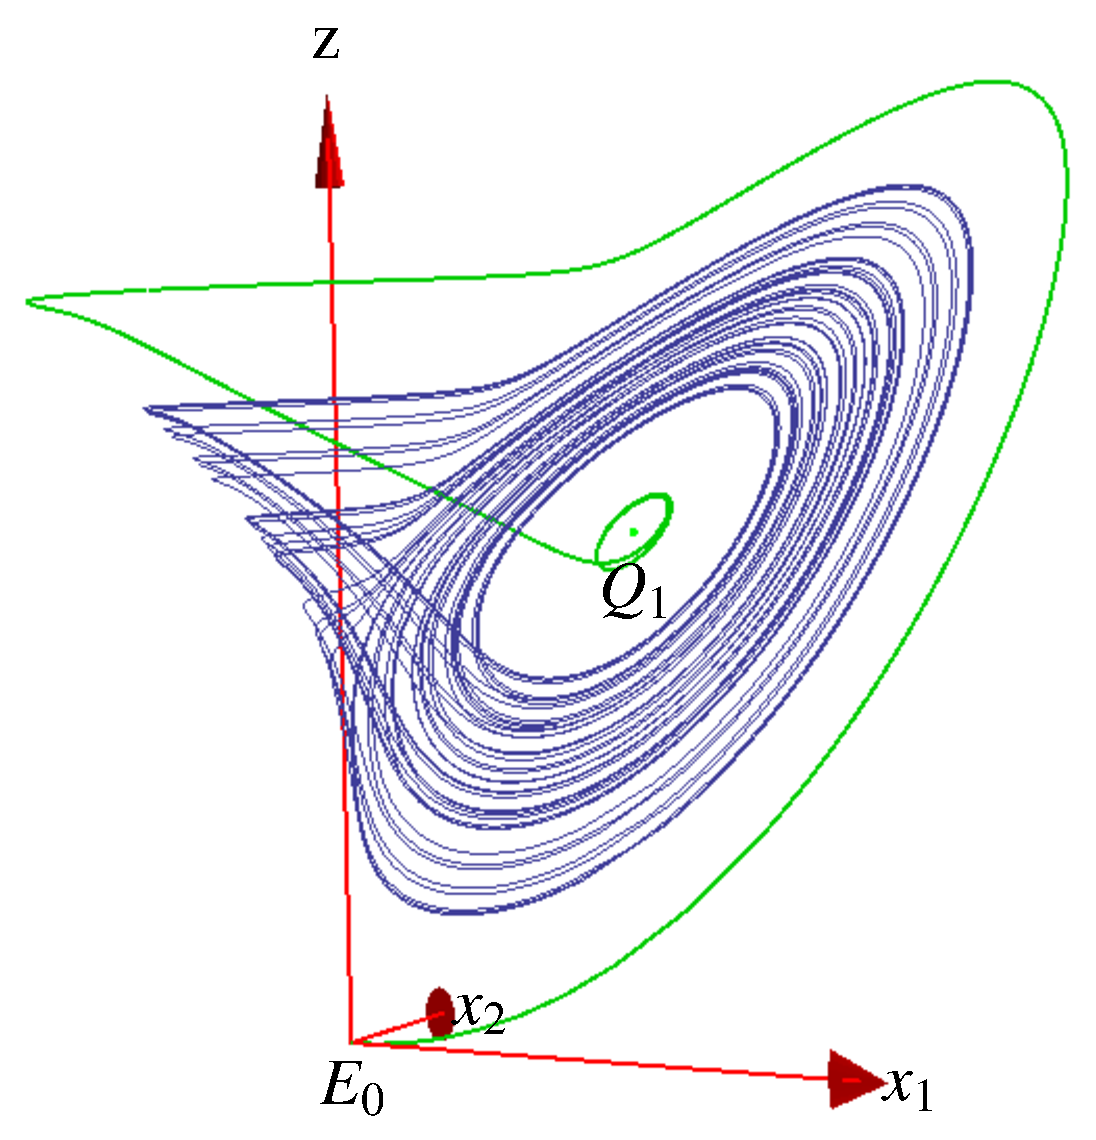
\includegraphics[width=0.43\textwidth]{../figs/CLEperpReqb1}
(b) 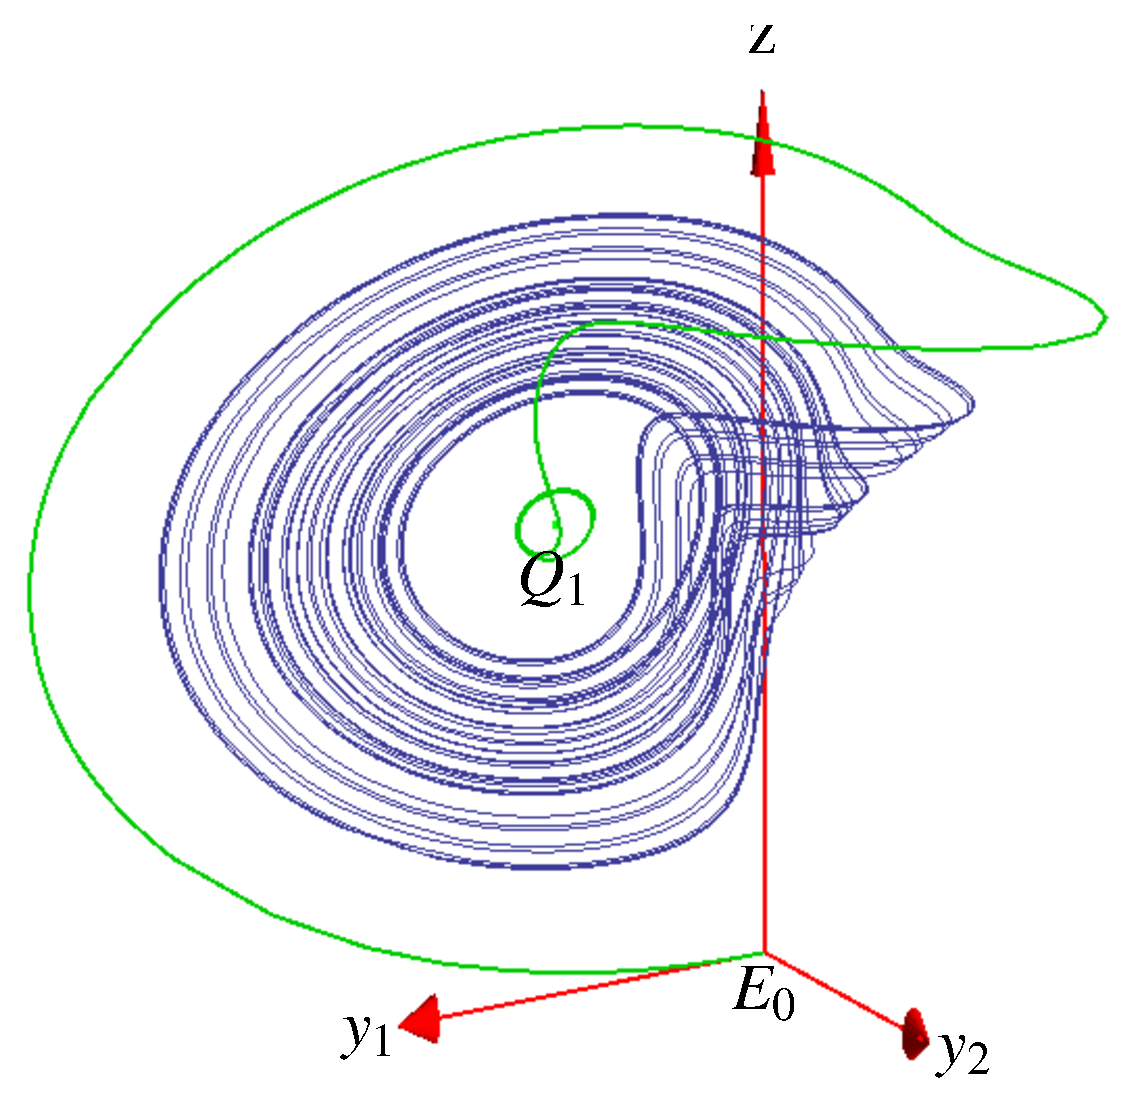
\includegraphics[width=0.43\textwidth]{../figs/CLEperpReqb}
\end{center}
\caption{
% ES removed this:
% {\Mframes}, \slice\ fixed by a point on the
% \reqv\ group orbit, $\slicep  = \ssp_{\REQB{1}}$. The strange
% attractor of \reffig{fig:CLE} in the \reducedsp\
% of \refeq{EqMotionMovFramePC}:
\Statesp\ portraits of \CLe\ dynamics for $e=1/10$,
$\ImrCLor=0$ in \reducedsp\ obtained by {\Mframes}, 
\slice\ fixed by a point on the
\reqv\ group orbit, $\slicep  = \ssp_{\REQB{1}}$.
(a) $\{x_1,x_2,z\}$ projection,
(b) $\{y_1,y_2,z\}$ projection.
}
\label{fig:CLEpcSect}
\end{figure}
%%%%%%%%%%%%%%%%%%%%%%%%%%%%%%%%%%%%%%%%%%%%%%%%%%%%%%%%%%%%%%%%
%
A long time trajectory of \refeq{EqMotionMovFramePC} with
$\slicep$ on the \reqv\ \REQB{1} group orbit is shown in
\reffig{fig:CLEpcSect}. Note that this figure is, not coincidentally,
identical to \reffig{fig:CLEmfReqb1}.
As initial condition we chose an initial point on the unstable manifold
of \REQB{1}, rotated back to the \slice\ by angle $\theta$ as
prescribed by \refeq{PCsectQ1}. 
% In \reffig{fig:CLEpcSect} we
% show the part of the trajectory for $t\in\left[70,100\right]$.
% The \reqv, now an equilibrium of the
% \reducedsp\ dynamics, organizes the flow into a R\"ossler type
% attractor. There appears to be no singularity in this
% attractor although we can run into trouble with
% \refeq{EqMotionMovFramePC} wherever the denominator in
% \refeq{MFdtheta} vanishes, \ie, the direction of group
% action on the point $\ssp$ is perpendicular to the direction
% of group action on $\slicep$.
    \PC{ in \reffig{fig:CLEpcSect}:\\
        * Mark $\ssp_{\REQB{}1}$ \\
        * Draw stable eigenvector of $\ssp_{\REQB{}1}$\\
        * State value of $\ssp_{\REQB{}1}$ somewhere
        }

A related method, the \emph{method of connections} is discussed
in the context of PDEs by Rowley \etal\rf{rowley_reduction_2003} but
is not adequate for the purpose of constructing return maps as 
the, so-called, \emph{geometric phase} is not factored out.
% \PublicPrivate{}{
% % %%%%%%%%%%%%%%%%%%%%%%%%%%%%%%%%%%%%%%%%%%%%%%%%%%
% % % computed by PCunrot.nb
% % \SFIG{PCunrot1}
% % {}{
% % {\Mframes}, continuous time version, for the
% % polar coordinates motivated $x^{*}=(0,1,0,0)$,
% % $x_1=0,\;x_2>0$, \slice. The \CLf\ strange attractor of
% % \reffig{fig:CLE} exhibits a discontinuity at
% % $x_2=0$ in the \reducedsp:
% % $\{x_2,y_2,z\}$ projection.
% % }
% % {fig:PCunrot1}
% % %%%%%%%%%%%%%%%%%%%%%%%%%%%%%%%%%%%%%%%%%%%%%%%%%%
% 
% Indeed, the method does encounter singularities in
% subsets of \statesp.
% For example, the \reducedsp\ equations \refeq{PCsectSin}
% for the polar coordinates inspired \slice\
% $x^{*}=(0,1,0,0)$, $x_1=0,\;x_2>0$,
% %this is illustrated by \reffig{fig:PCunrot}.
% %$(\rho_1,\theta_1)$ are polar coordinates, $\rho_1 =
% %\sqrt{\ssp_1^{ 2} + \ssp_2^{2}}$, see \refeq{eq:CartToPol},
% are given by
% \beq
% \dot{\ssp} = \vel - \frac{\vel_1}{\ssp_2} \Lg \cdot \ssp
% \,.
% \ee{EqMotionMovFrame}
% A typical trajectory is shown in \reffig{fig:PCunrot}.
%    \PC{this is not \reffig{fig:PCunrot} - copy correct fig
%        from wilczak/blog
%        }
% The problem with defining the \slice\ by
% \refeq{EqMotionMovFrame} is apparently that it fixes rotations
% in the $(\ssp_1,\ssp_2)$ plane, not the full 4\dmn\ space.
% }

\renewcommand{\Group}{\ensuremath{\Gamma}}    % Siminos Lie group
